
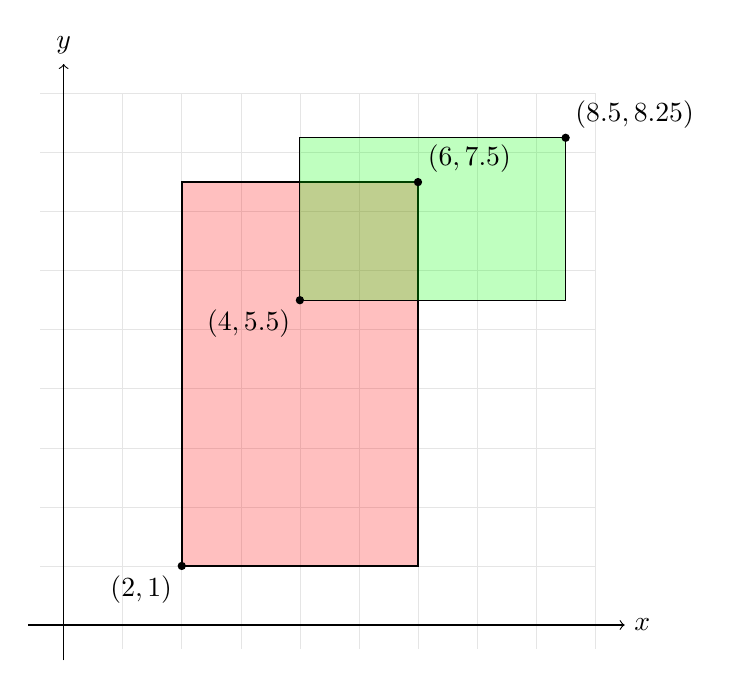
\begin{tikzpicture}[scale=0.75]
  \draw[step=1.0cm,black!10!white,very thin] (-0.4,-0.4) grid (9,9); %
  \draw[->] (-0.6,0) -- (9.5,0) node[right] {$x$};%
  \draw[->] (0,-0.6) -- (0,9.5) node[above] {$y$};%

  \filldraw[fill=red,thick,fill opacity=.25] (2, 1) rectangle (6, 7.5);
  \filldraw[fill=green,fill opacity=.25] (4, 5.5) rectangle (8.5, 8.25);

  \fill (2, 1) circle (2pt);
  \fill (6, 7.5) circle (2pt);
  \fill (4, 5.5) circle (2pt);
  \fill (8.5, 8.25) circle (2pt);

  \node [] (A) at (2, 1) [below left] {$(2, 1)$};
  \node [] (B) at (6, 7.5) [above right] {$(6, 7.5)$};
  \node [] (C) at (4, 5.5) [below left] {$(4, 5.5)$};
  \node [] (D) at (8.5, 8.25) [above right] {$(8.5, 8.25)$};

\end{tikzpicture}
